\subsubsection{Double Exponent Model}

In this model, we have two variables: \\
\begin{enumerate}
    \item $v(t)$ represents the membrane potential of the neuron

    \item $I(t)$ represents the synaptic current.
\end{enumerate}

The term $\tau_m$ is the membrane time constant, and $\tau_s$ is the synaptic time constant. Both time constants determine how quickly the variables respond to changes in input.

The second-order low-pass filter model is represented by the following equations:

\begin{equation} \label{eq:def_eq_I}
    I(t) + \tau_s \frac{dI(t)}{dt} = I_{\text{in}}(t)
\end{equation}

\begin{equation} \label{eq:def_eq_V}
    v(t) + \tau_m \frac{dv(t)}{dt} = I(t)
\end{equation}

This model is motivated by the desire to capture more realistic neuronal dynamics. The first equation \ref{eq:def_eq_I} represents the dynamics of the input synaptic current, where $\tau_s$ controls how quickly the current responds to changes in input. The second equation \ref{eq:def_eq_V} represents the dynamics of the neuron's membrane potential, where $\tau_m$ determines the speed of the response to synaptic input.

\subsubsection*{Spike Response:}

To understand the spike response, let's consider the case of an impulse input current $I_{\text{in}}(t) = I_0 \delta(t)$ , where $I_0$ is the amplitude of the input current and $\delta(t)$ is the Dirac delta function.

In this case, the equations become:

\begin{equation} \label{eq:I_spike_res}
    I(t) + \tau_s \frac{dI(t)}{dt} = I_0 \delta(t)
\end{equation}

\begin{equation} \label{eq:V_spike_res}
    v(t) + \tau_m \frac{dv(t)}{dt} = I(t)
\end{equation}

Solving Equation \ref{eq:I_spike_res}: \\
We can solve Equation \ref{eq:I_spike_res} by taking the Laplace transform. The Laplace transform of the Dirac delta function as input is:

\begin{equation}
    I(s) + \tau_s s I(s) = I_0
\end{equation}

Solving for $I(s)$:

\begin{equation}
    I(s) = \frac{I_0}{1 + \tau_s s}
\end{equation}

Solving Equation \ref{eq:V_spike_res}: \\
Similarly, we take the Laplace transform of Equation \ref{eq:V_spike_res}:

\begin{equation}
    v(s) + \tau_m s v(s) = I(s)
\end{equation}

Substitute the expression for $I(s)$:

\begin{equation}
    v(s) + \tau_m s v(s) = \frac{I_0}{1 + \tau_s s}
\end{equation}

Solving for $v(s)$:

To obtain the time-domain solution from the Laplace domain, we use the method of partial fraction decomposition to rewrite the Laplace-domain expression in a form that allows us to take the inverse Laplace transform.

From Equation (10) in the previous response:

\begin{equation}
    v(s) = \frac{I_0}{(1 + \tau_s s)(1 + \tau_m s)}
\end{equation}

To decompose this expression into partial fractions, we need to find constants $A$ and $B$ such that:

\begin{equation}
    \frac{I_0}{(1 + \tau_s s)(1 + \tau_m s)} = \frac{A}{1 + \tau_s s} + \frac{B}{1 + \tau_m s}
\end{equation}

Now, we can find the values of $A$ and $B$ by equating the numerators:

\begin{equation}
    I_0 = A(1 + \tau_m s) + B(1 + \tau_s s)
\end{equation}

For simplicity, we can let $s = 0$ to find the value of $A$:

\begin{equation}
    I_0 = A
\end{equation}

Next, we can let $s = -\frac{1}{\tau_s}$ to find the value of $B$:

\begin{equation}
    I_0 = B\left(1 - \frac{\tau_s}{\tau_m}\right)
\end{equation}

Solving for $B$:

\begin{equation}
    B = \frac{I_0}{1 - \frac{\tau_s}{\tau_m}} = \frac{I_0}{\frac{\tau_m - \tau_s}{\tau_m}} = \frac{I_0 \tau_m}{\tau_m - \tau_s}
\end{equation}

Now that we have the values of $A$ and $B$, we can rewrite the Laplace-domain expression in terms of partial fractions:

\begin{equation}
    v(s) = \frac{I_0}{(1 + \tau_s s)(1 + \tau_m s)} = \frac{I_0}{\tau_m - \tau_s} \left(\frac{\tau_m}{1 + \tau_m s} - \frac{\tau_s}{1 + \tau_s s}\right)
\end{equation}

To take the inverse Laplace transform, we use standard Laplace transform pairs. The inverse Laplace transform of $\frac{\tau_m}{1 + \tau_m s}$ is $e^{-\frac{t}{\tau_m}}$, and the inverse Laplace transform of $\frac{\tau_s}{1 + \tau_s s}$ is $e^{-\frac{t}{\tau_s}}$. Thus, the time-domain solution for the membrane potential $v(t)$ is:

\begin{equation}
    v(t) = \frac{I_0}{\tau_m - \tau_s} \left(e^{-\frac{t}{\tau_m}} - e^{-\frac{t}{\tau_s}}\right)
\end{equation}

This is the double exponential spike response of the neuron's membrane potential to an impulse input current $I_{\text{in}}(t) = I_0 \delta(t)$. \\
The solution is characterized by two time constants: $\tau_m$ and $\tau_s$. The first term with $\tau_m$ dominates at short timescales, representing the fast response of the neuron, while the second term with $\tau_s$ governs the slower response at longer timescales.

We can normalize it into:

\begin{equation}
    v(t) = v_0 \cdot (e^{-t/\tau_m} - e^{-t/\tau_s})
\end{equation}

\begin{figure}[H]
    \centering
    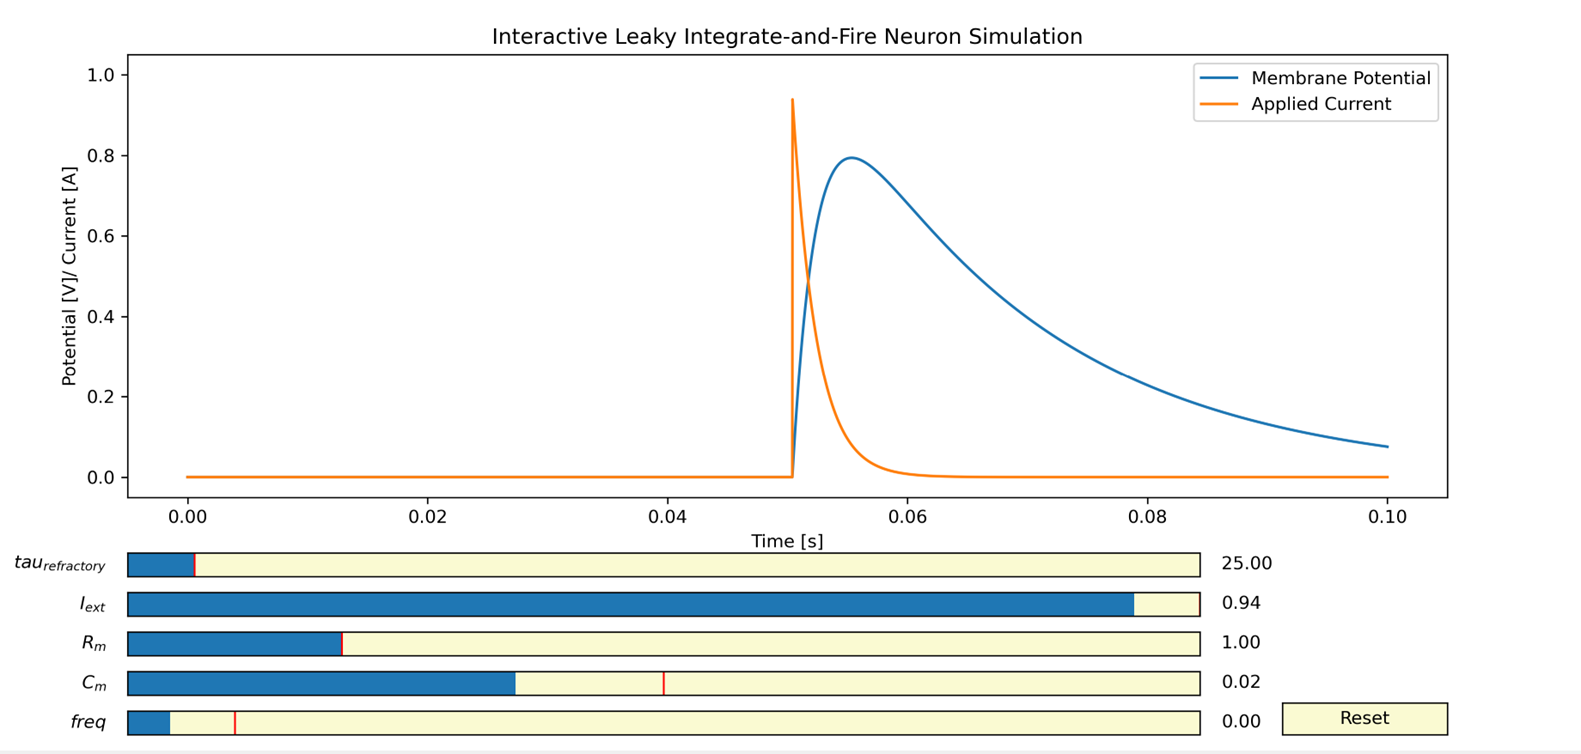
\includegraphics[width=0.6\textwidth]{scientific-background/computational-models/LIF/graphs/LIF-second-order.png}
    \caption{LIF 2-order membrane voltage response to spike}
    \label{fig:LIF-second-order}
\end{figure}

A useful definition will be:

\begin{equation}
    k(t) = v_0 \cdot (e^{-t/\tau_m} - e^{-t/\tau_s})
\end{equation}

So, the solution for:

\begin{equation}
    v(t) = \sum_{t^l} k(t - t^l)
\end{equation}

\begin{figure}[H]
    \centering
    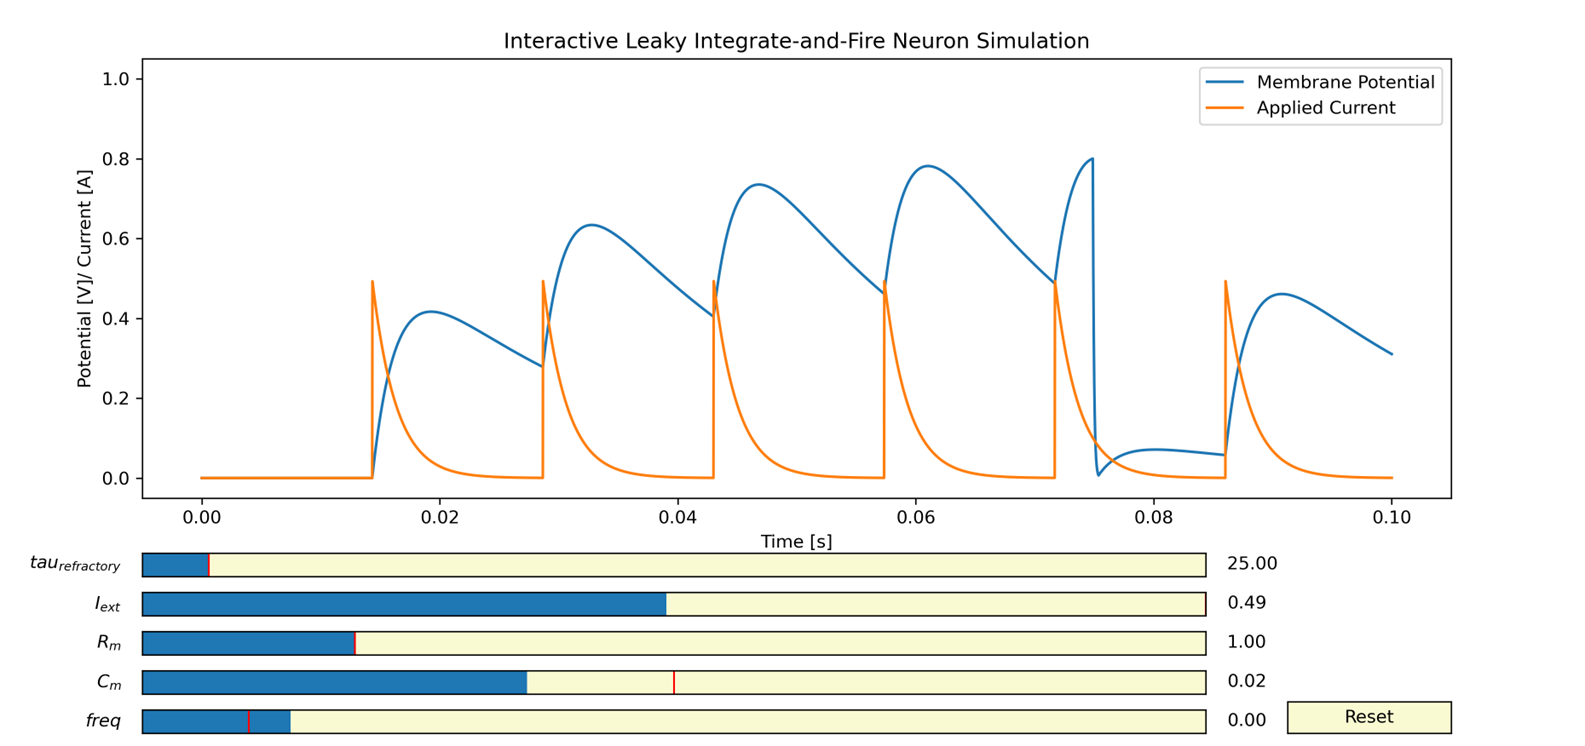
\includegraphics[width=0.6\textwidth]{scientific-background/computational-models/LIF/graphs/LIF-spike-response-second-order.png}
    \caption{LIF 2-order membrane voltage response to multiple spikes}
    \label{fig:LIF-second-order-spike-response}
\end{figure}
